%Copyright 2019 Christopher M. Jermaine (cmj4@rice.edu) and Risa B. Myers (rbm2@rice.edu)
%
%Licensed under the Apache License, Version 2.0 (the "License");
%you may not use this file except in compliance with the License.
%You may obtain a copy of the License at
%
%    https://www.apache.org/licenses/LICENSE-2.0
%
%Unless required by applicable law or agreed to in writing, software
%distributed under the License is distributed on an "AS IS" BASIS,
%WITHOUT WARRANTIES OR CONDITIONS OF ANY KIND, either express or implied.
%See the License for the specific language governing permissions and
%limitations under the License.
%===============================================================
\documentclass[aspectratio=169]{beamer}
\mode<presentation> 
{
\usetheme[noshadow, minimal,numbers,riceb,nonav]{Rice}
\usefonttheme[onlymath]{serif}
\setbeamercovered{transparent}
}
\useinnertheme{rectangles}

\usepackage[english]{babel}

\usepackage{mathptmx}
\usepackage{helvet}
\usepackage{courier}
\usepackage[T1]{fontenc}
\usepackage{trajan}

\setbeamerfont{block body}{size=\tiny}
\usepackage{listings}

\newenvironment{noindentitemize}
{ \begin{itemize}
 \setlength{\itemsep}{1.5ex}
  \setlength{\parsep}{0pt}   
  \setlength{\parskip}{0pt}
 \addtolength{\leftskip}{-2em}
 }
{ \end{itemize} }

\newenvironment{noindentitemize2}
{ \begin{itemize}
  \setlength{\itemsep}{0ex}
  \setlength{\parskip}{0pt}
  \setlength{\parsep}{0pt}   
  \addtolength{\leftskip}{-2em}  }
{ \end{itemize} }


%===============================================================%
\title[]
{Tools \& Models for Data Science}

\subtitle{Support Vector Machines}

\author[]{Chris Jermaine \& Risa Myers}
\institute
{
  Rice University
}

\date[]{}

\subject{Beamer}


\begin{document}
\begin{frame}
 \titlepage
\end{frame}


%***********************************************************
\begin{frame}{ML Roadmap}

\begin{itemize}
	\item Linear Regression
	\item Generalized Linear Models
\end{itemize}
\end{frame}
%***********************************************************
\begin{frame}{Alternatives to Logistic Regression}

\begin{itemize}
	\item The ``Big Three'' for classification
        \begin{itemize}
                \item Logistic regression
		\item Support Vector Machines
		\item kNN
        \end{itemize}
\end{itemize}
\end{frame}
%***********************************************************
\begin{frame}{Recall: Logistic Regression}

\begin{itemize}
\item Specialized case of GLM
\item Where the error can come from a family of distributions
\item If we use the Bernoulli distribution
\begin{itemize}
\item We get Logistic Regression
\item There is a different, but mathematically equivalent representation of Logistic Regression using the sigmoid function
\end{itemize}
\end{itemize}
\centering{
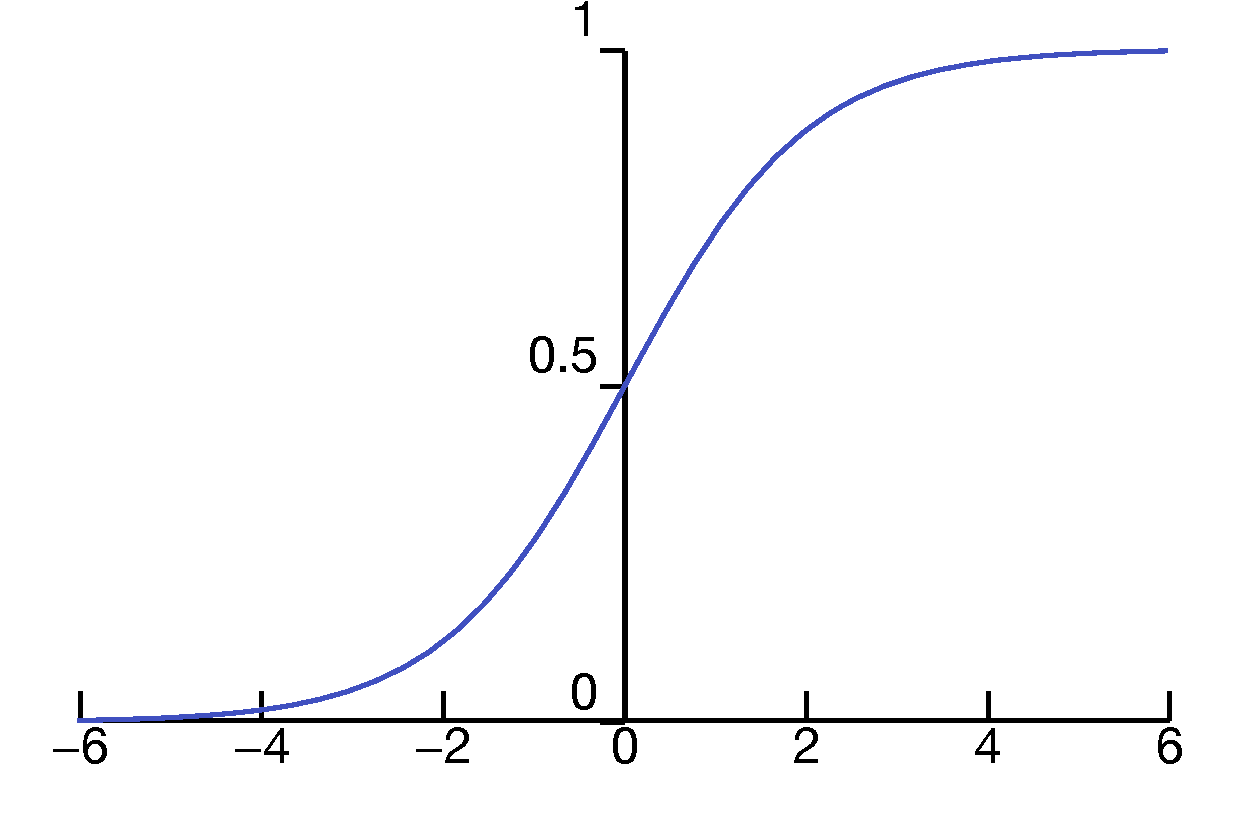
\includegraphics[width=.25\textwidth]{lectSVM/Logistic-curve.pdf}
}
\end{frame}
%***********************************************************
\begin{frame}{The Sigmoid Function}

\begin{columns}
\begin{column}{0.5\textwidth}
\begin{itemize}
\item $S(x) = \frac{1}{1+e^{-x}} = \frac{e^x}{e^x + 1}$
\item There are others (Hyperbolic tangent, Arctangent, ...)
\item Key properties
\begin{itemize}
\item Monotonic
\item ``S'' shape
\item Horizontal asymptotes
\end{itemize}
\end{itemize}
\end{column}
\begin{column}{0.5\textwidth}
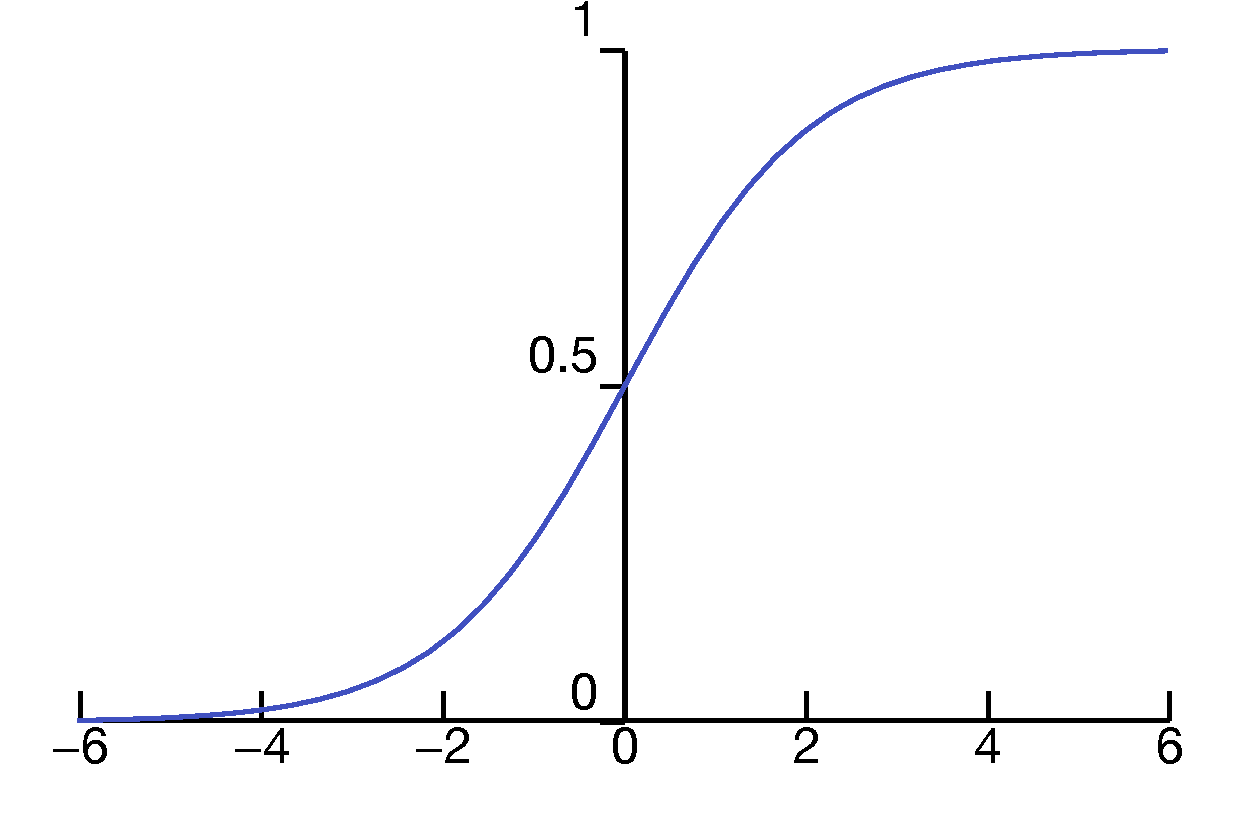
\includegraphics[width=1\textwidth]{lectSVM/Logistic-curve.pdf}
\end{column}
\end{columns}
\end{frame}
%***********************************************************
\begin{frame}{Training and Inference}

\begin{itemize}
\item During training
\begin{itemize}
\item During training we have a set of $n\ \{x_i, y_i\}$ pairs
\item We use a method (MLE, gradient ascent, etc.) to learn the vector of regression coefficients, $r$
\item To maximize the log likelihood function
$$\sum_i y_i (x_i \cdot r) - \log (1 + e^{x_i \cdot r})$$
\end{itemize}
\item During inference
\begin{itemize}
\item We use $r$ and the new $x_i$s to choose the label,  $y_i$, to maximize the LLH
\item $y_i$ in $\{0,1\}$
%\item Plug in both possible values for $y_i$
\item Basically, if $x_i \cdot r < 0$, pick $y_i = 0$
\end{itemize}
\end{itemize}
\end{frame}
%***********************************************************
\begin{frame}{Human Logistic Regression}

\begin{columns}
\begin{column}{0.6\textwidth}
\begin{itemize}
\item When the data are ``linearly separable''
	\begin{itemize}
	\item Recall
	$$LLH = \sum_i y_i (x_i \cdot r) - \log (1 + e^{x_i \cdot r})$$
	\item Where $x_i$ are the training data
	\item $r$ is the vector of regression coefficients
	\item $y_i = sign(x_i \cdot  r)$
	\item Where $sign(x_i \cdot r) = $
	$\begin{cases} 1 & \textrm{if }x_i \cdot r > 0 \\
	 0 & \textrm{if } x_i \cdot r < 0 \\
	 \end{cases}$
	\item Assigns a class based on which side of the ``cutting" line the point is on
	\item[?] Where does the cutting line go?
	\end{itemize}
\end{itemize}
\end{column}
\begin{column}{0.4\textwidth}
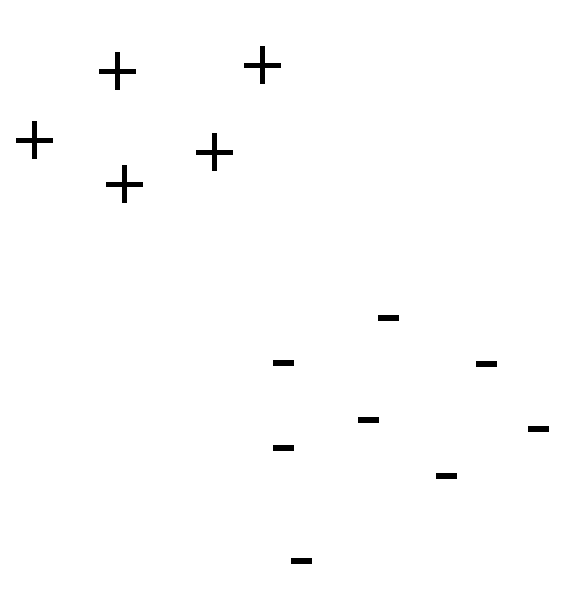
\includegraphics[width=1\textwidth]{lectSVM/logR0.pdf}
\end{column}
\end{columns}
\end{frame}
%***********************************************************
\begin{frame}{Humans vs. Machine Logistic Regression}

\begin{columns}
\begin{column}{0.5\textwidth}
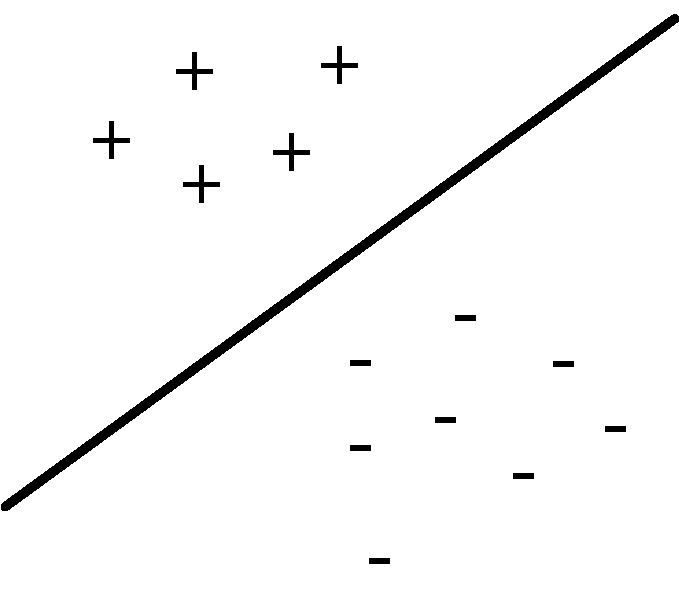
\includegraphics[width=.85\textwidth]{lectSVM/logR1.pdf}
\end{column}
\begin{column}{0.5\textwidth}
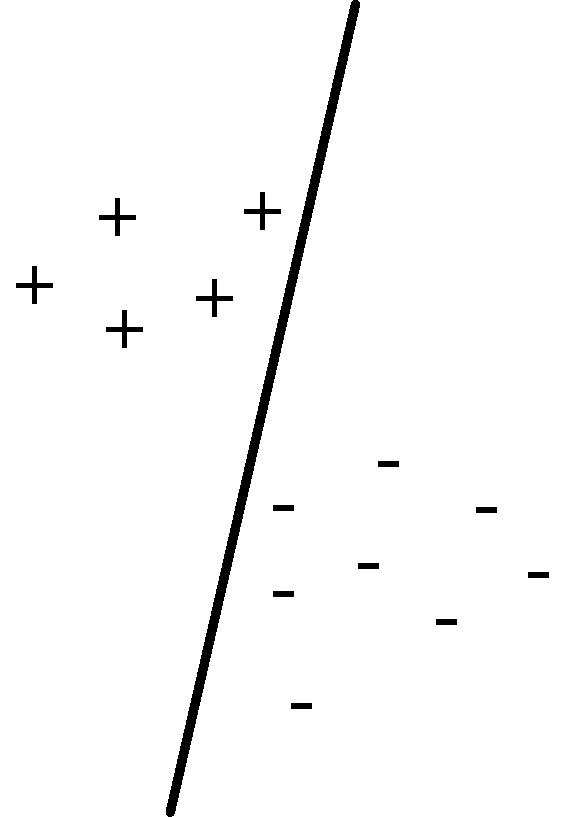
\includegraphics[width=.7\textwidth]{lectSVM/logRegBoundary.pdf}
\end{column}
\end{columns}
\end{frame}
%***********************************************************
\begin{frame}{Humans vs. Machine Logistic Regression}

\begin{columns}
\begin{column}{0.5\textwidth}
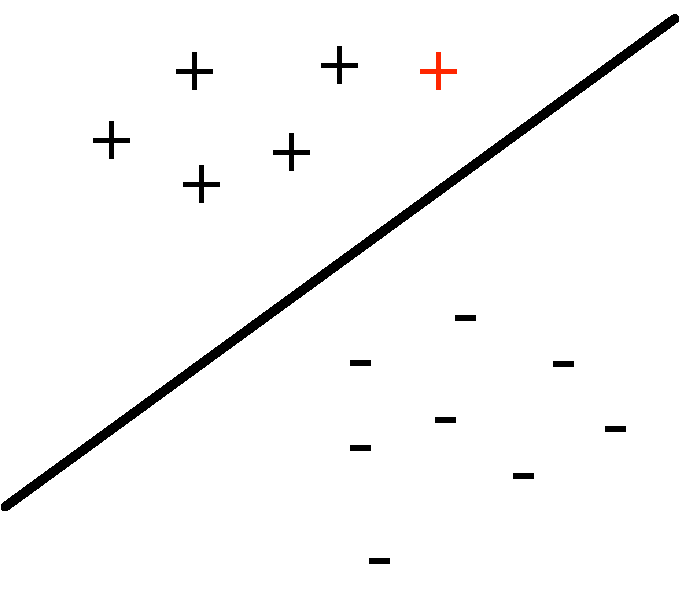
\includegraphics[width=.85\textwidth]{lectSVM/logR1HumanAddPt.pdf}
\end{column}
\begin{column}{0.5\textwidth}
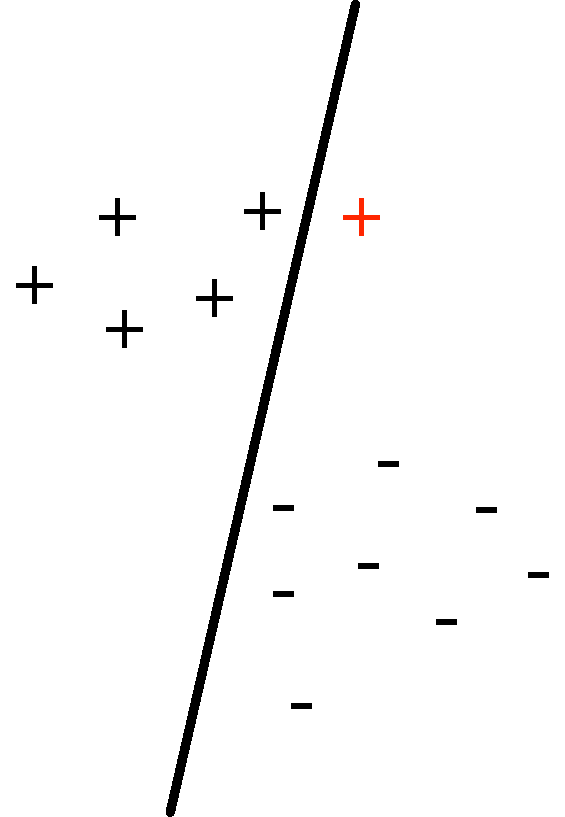
\includegraphics[width=.7\textwidth]{lectSVM/logR1addPt.pdf}
\end{column}
\end{columns}
\end{frame}
%***********************************************************
\begin{frame}{Problem With Un-Regularized Logistic Regression}

\begin{columns}
\begin{column}{0.6\textwidth}
	\begin{itemize}
	\item Possible to choose infinite models that get infinite LLH
	\item Just choose ANY cutting plane between classes
	\item That is, choose any $r$ that perfectly classifies data, so $y_i = sign (x_i \cdot r)$
	\item Then use $r' = BIG \times r$
	\item And $\sum_i y_i (x_i \cdot r') - \log (1 + e^{x_i \cdot r'})$ will be really big
	\item  Infinitely many models give infinite LLH
	\item Bad: Not clear which plane is preferred
	\end{itemize}
\end{column}
\begin{column}{0.4\textwidth}
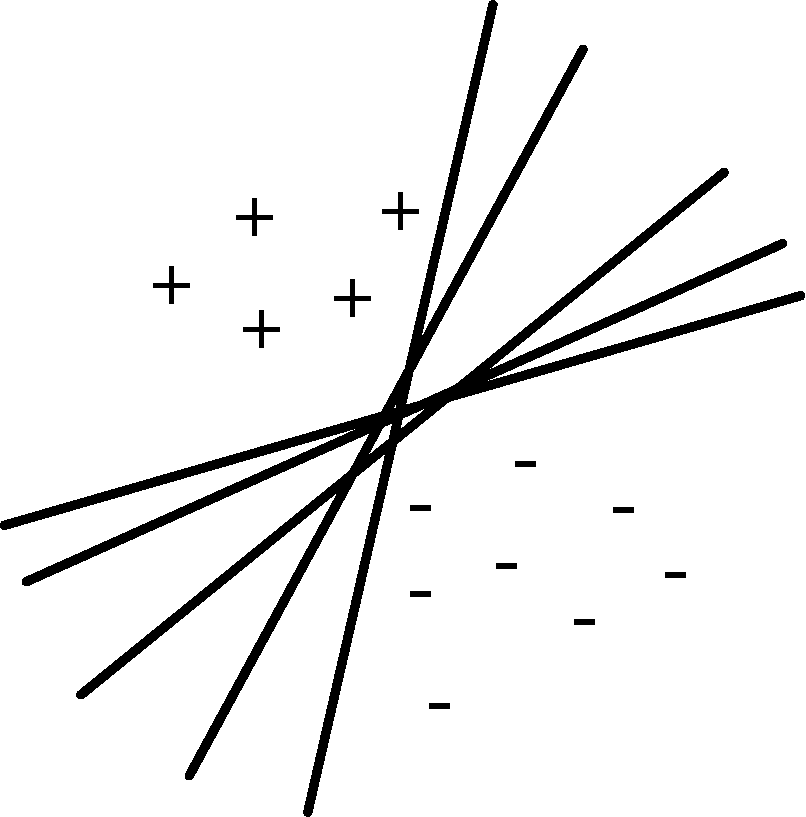
\includegraphics[width=1\textwidth]{lectSVM/logRMany.pdf}
\end{column}
\end{columns}
\end{frame}
%***********************************************************
\begin{frame}{SVMs: Geometric, Not Probabilistic}

\begin{columns}
\begin{column}{0.6\textwidth}
\begin{itemize}
\item What should a classifier do in this super-easy case?
\begin{itemize}
\item Just put the widest strip possible between two classes
\item Future points above center of strip are ``yes''
\item Below center of strip are ``no''
\item Points that keep strip from expanding are ``support vectors''
\end{itemize}
\end{itemize}
\end{column}
\begin{column}{0.4\textwidth}
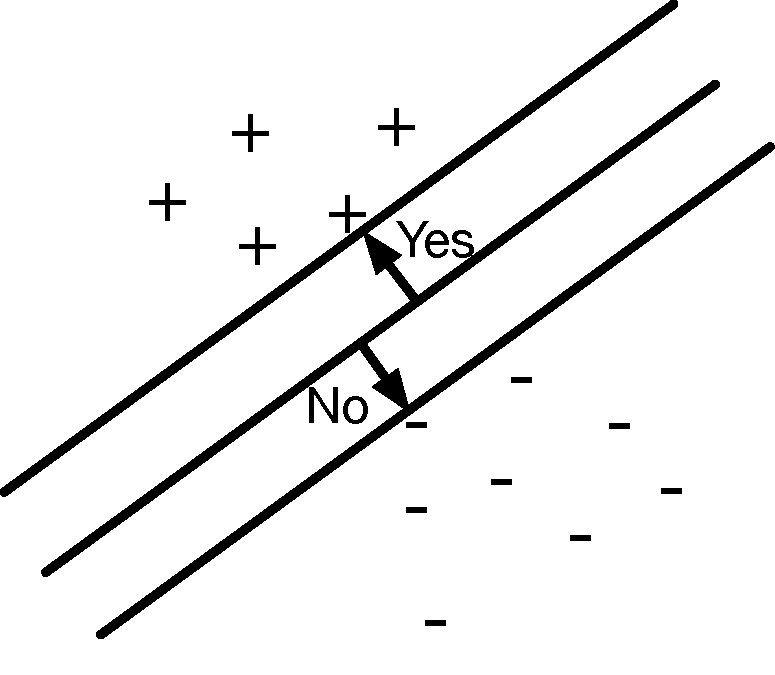
\includegraphics[width=1\textwidth]{lectSVM/logRstrip.pdf}
\end{column}
\end{columns}
\end{frame}
%***********************************************************
\begin{frame}{SVMs Steps 1}

\begin{columns}[T]
\begin{column}{0.6\textwidth}
\begin{enumerate}
\item  Choose an arbitrary, infinitely thin cutting plane
\end{enumerate}
\end{column}
\begin{column}{0.4\textwidth}
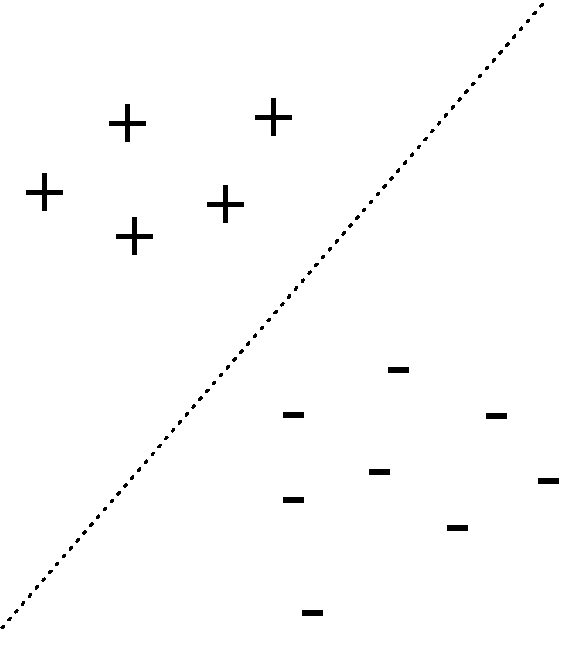
\includegraphics[width=1\textwidth]{lectSVM/svm1}
\end{column}
\end{columns}
\end{frame}
%***********************************************************
\begin{frame}{SVMs Steps 2}

\begin{columns}[T]
\begin{column}{0.6\textwidth}
\begin{enumerate}
\item  Choose an arbitrary, infinitely thin cutting plane
\item Make it wider
\end{enumerate}
\end{column}
\begin{column}{0.4\textwidth}
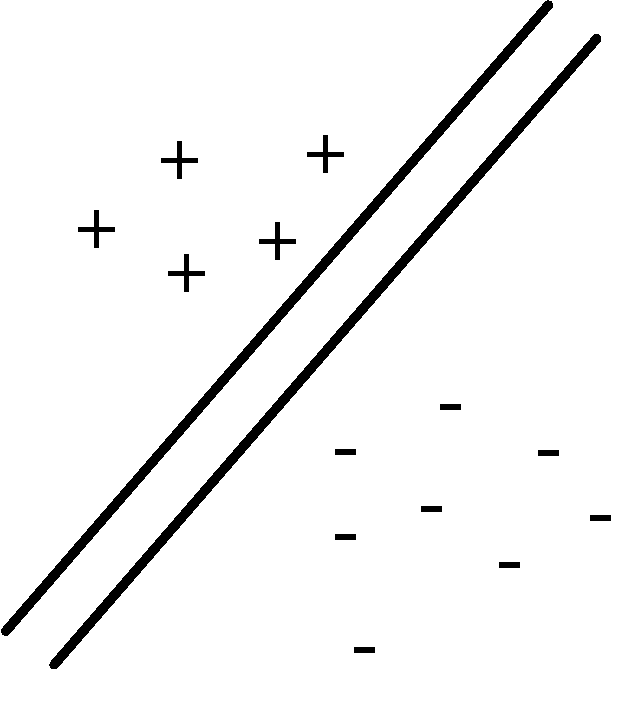
\includegraphics[width=1\textwidth]{lectSVM/svm2}
\end{column}
\end{columns}
\end{frame}
%***********************************************************
\begin{frame}{SVMs Steps 3}

\begin{columns}[T]
\begin{column}{0.6\textwidth}
\begin{enumerate}
\item  Choose an arbitrary, infinitely thin cutting plane
\item Make it wider
\item Keep widening until you hit a data point
\end{enumerate}
\end{column}
\begin{column}{0.4\textwidth}
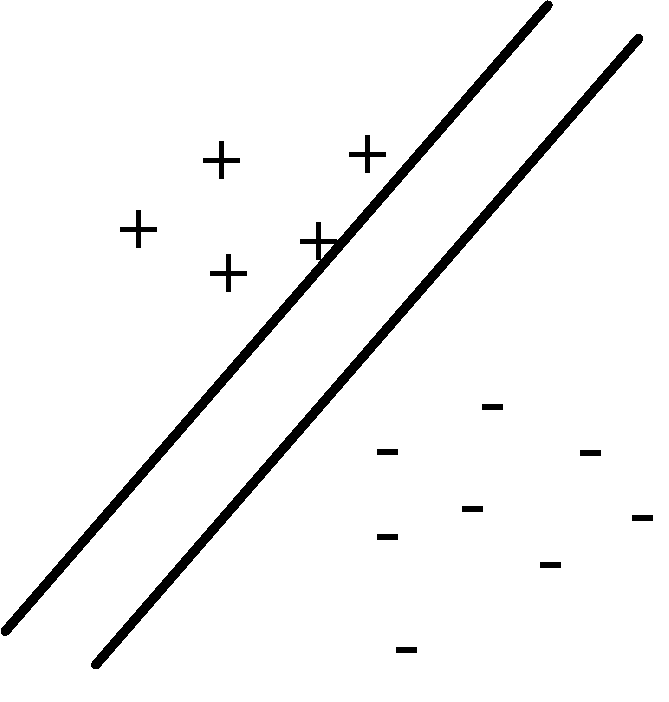
\includegraphics[width=1\textwidth]{lectSVM/svm3}
\end{column}
\end{columns}
\end{frame}
%***********************************************************
\begin{frame}{SVMs Steps 3}

\begin{columns}[T]
\begin{column}{0.6\textwidth}
\begin{enumerate}
\item  Choose an arbitrary, infinitely thin cutting plane
\item Make it wider
\item Keep widening until you hit a data point, rotating if needed
\end{enumerate}
\end{column}
\begin{column}{0.4\textwidth}
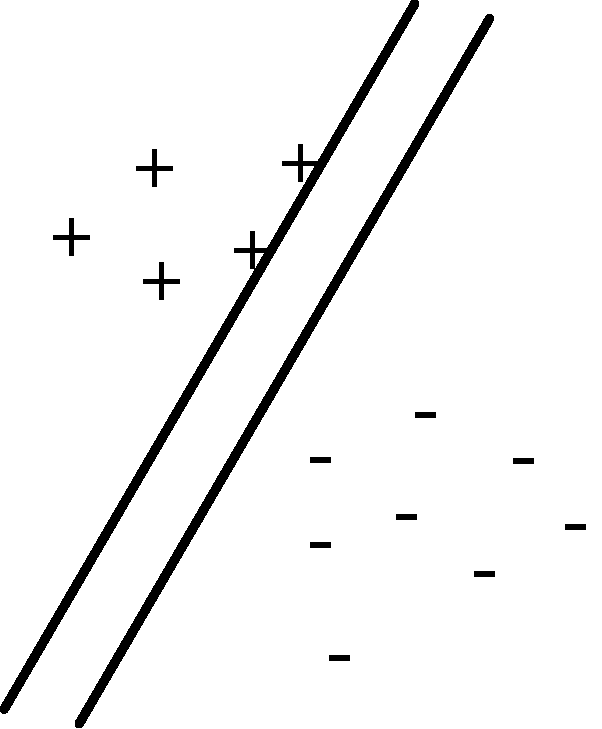
\includegraphics[width=1\textwidth]{lectSVM/svm4}
\end{column}
\end{columns}
\end{frame}

%***********************************************************
\begin{frame}{SVMs Steps 4}

\begin{columns}[T]
\begin{column}{0.6\textwidth}
\begin{enumerate}
\item  Choose an arbitrary, infinitely thin cutting plane
\item Make it wider
\item Keep widening until you hit a data point, rotating if needed
\item Expand in the other direction
\end{enumerate}
\end{column}
\begin{column}{0.4\textwidth}
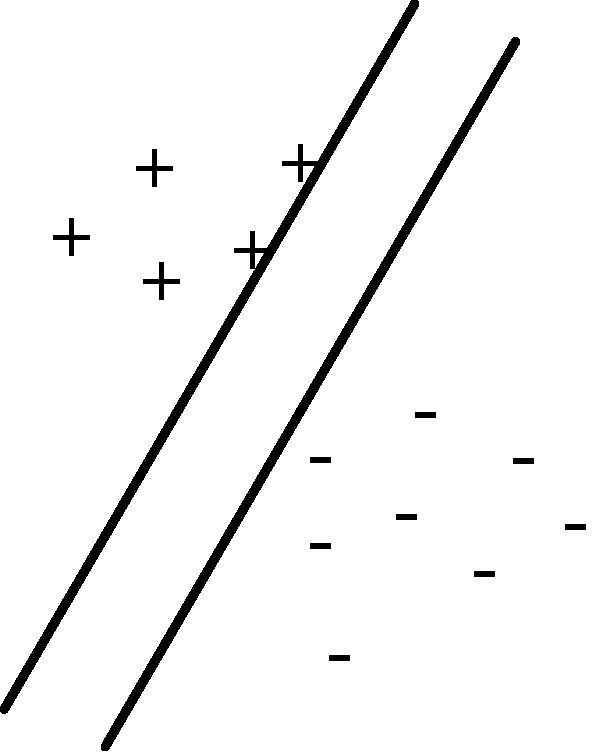
\includegraphics[width=1\textwidth]{lectSVM/svm5}
\end{column}
\end{columns}
\end{frame}
%***********************************************************
\begin{frame}{SVMs Steps 4}

\begin{columns}[T]
\begin{column}{0.6\textwidth}
\begin{enumerate}
\item  Choose an arbitrary, infinitely thin cutting plane
\item Make it wider
\item Keep widening until you hit a data point, rotating if needed
\item Expand in the other direction
\end{enumerate}
\end{column}
\begin{column}{0.4\textwidth}
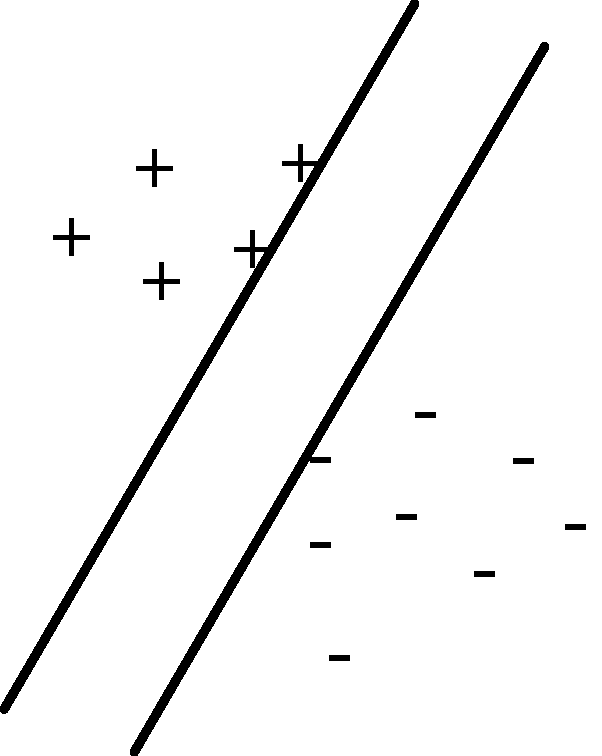
\includegraphics[width=1\textwidth]{lectSVM/svm6}
\end{column}
\end{columns}
\end{frame}


%***********************************************************
\begin{frame}{SVMs Steps 5 \& 6}

\begin{columns}[T]
\begin{column}{0.6\textwidth}
\begin{enumerate}
\item  Choose an arbitrary, infinitely thin cutting plane
\item Make it wider
\item Keep widening until you hit a data point, rotating if needed
\item Expand in the other direction
\item Stop when strip is wedged in by three points
\item Choose the line in the center of the strip
\end{enumerate}
\end{column}
\begin{column}{0.4\textwidth}
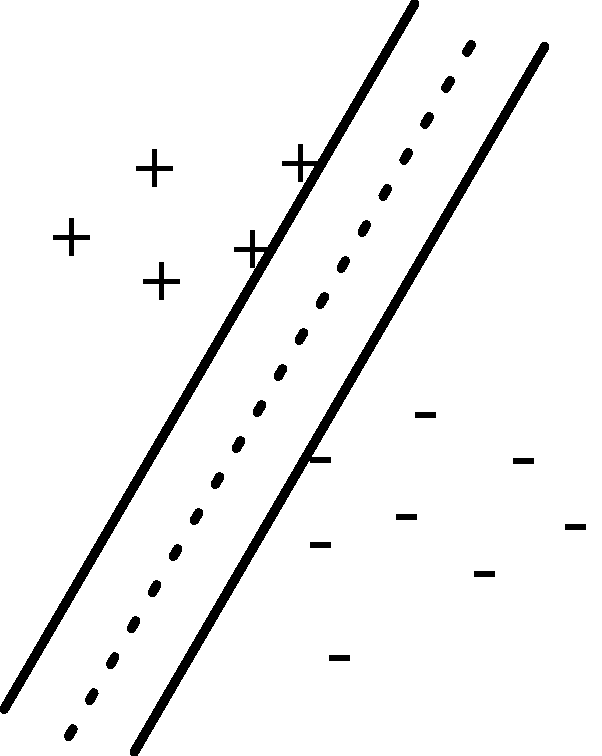
\includegraphics[width=1\textwidth]{lectSVM/svm7}
\end{column}
\end{columns}
\end{frame}

%***********************************************************
\begin{frame}{Basic Formulation}

\begin{itemize}
\item Idea: We want to describe this geometric algorithm mathematically
\item Any line/plane/hyperplane can be described by a normal vector $w$ and a distance $b$
	\begin{itemize}
	\item The line/plane/hyperplane is all points $x$ where $w \cdot x - b = 0$
	\item $d$ is the number of dimensions of our data
	\item $w$ is a $d$ dimensional vector
	\item $b$ is an intercept term
	\end{itemize}
\end{itemize}
\end{frame}
%***********************************************************
\begin{frame}{Basic Formulation}

\begin{itemize}
\item SVM chooses two parallel planes 
$$w \cdot x - b = 1$$ 
$$w \cdot x - b = -1$$
\item NOTE: Notation change from $\{0, 1\}$ to $\{-1, 1\}$ for mathematical convenience
\item We need to learn $w$ and $b$
\end{itemize}
\end{frame}
%***********************************************************
\begin{frame}{Basic Formulation}

\begin{itemize}
\item SVM chooses two parallel planes 
$$w \cdot x - b = 1$$ 
$$w \cdot x - b = -1$$
\item We need to learn $w$ and $b$
\item This is a constrained maximization problem
	\begin{itemize}
	\item Use $||w||$ to denote the $l_2$ norm of the vector $w$ % this is the distance between the planes
	\item Can prove distance between them is $\frac{2}{||w||}$
	\end{itemize}
\item Where $w \cdot x_i - b \geq 1$ when $x_i$ is ``yes''
\item Where $w \cdot x_i - b \leq -1$ when $x_i$ is ``no''
	\begin{itemize}
	\item in general, where $y_i (w \cdot x_i - b) \geq 1$
	\end{itemize}
\end{itemize}
\end{frame}
%***********************************************************
\begin{frame}{Basic Formulation}

\begin{itemize}
\item SVM chooses two parallel planes 
$$w \cdot x - b = 1$$ 
$$w \cdot x - b = -1$$
\item We need to learn $w$ and $b$
\item This is a constrained maximization problem
\item Where $w \cdot x_i - b \geq 1$ when $x_i$ is ``yes''
\item Where $w \cdot x_i - b \leq -1$ when $x_i$ is ``no''
	\begin{itemize}
	\item in general, where $y_i (w \cdot x_i - b) \geq 1$
	\end{itemize}
\item We want to maximize  $\frac{2}{||w||}$ subject to the constraint above
	\begin{itemize}
	\item One class is above the plane
	\item The other class is below the plane
	\end{itemize}
\end{itemize}
\end{frame}
%***********************************************************
\begin{frame}{Basic Formulation}

\begin{itemize}
\item In the end we have...
\item Choose $w$ to maximize $\frac{2}{||w||}$ (alt., to minimize $||w||$)
\item Subject to $y_i (w \cdot x_i - b) \geq 1$
\item That's all a SVM is!
\item Easily written as a quadratic program (objective function quadratic)
\begin{itemize}
\item However, quadratic programs are NP-Hard
\item There are solvers out there
\item But, SVMs are a limited version of the quadratic program, so it's not that hard
\end{itemize}
\end{itemize}
\end{frame}
%***********************************************************
\begin{frame}{What does NP-Hard Mean?}

\begin{itemize}
\item Computational complexity 
\item COMP 182/382/482 material
\item Has to do with how much time it takes to solve the problem
\item Non-deterministic polynomial time hardness
\end{itemize}
\end{frame}
%***********************************************************
\begin{frame}{One Issue: What If the Data Are Not Linearly Separable?}

\begin{columns}
\begin{column}{0.6\textwidth}
\begin{itemize}
\item Then no solution to above problem!
\item In other words, our ``Subject to'' clause may result in ZERO solutions
\item Subject to $y_i (w \cdot x_i - b) \geq 1$
\item[?] How do we handle this?
\end{itemize}
\end{column}
\begin{column}{0.4\textwidth}
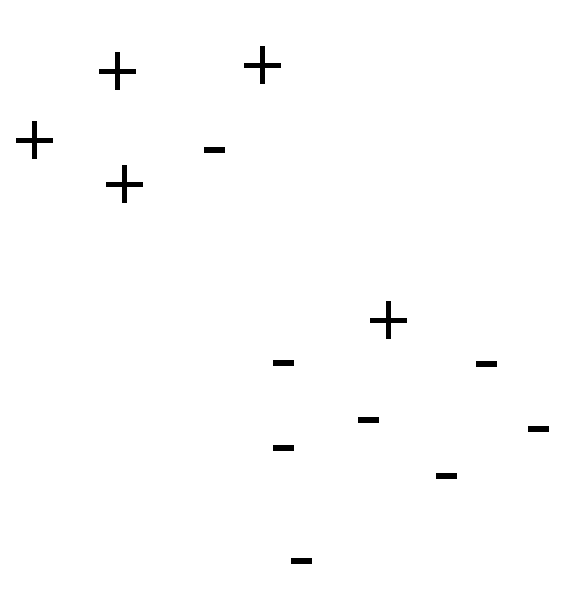
\includegraphics[width=1\textwidth]{lectSVM/nonLinSep.pdf}
\end{column}
\end{columns}

\end{frame}
%***********************************************************
\begin{frame}{One Issue: What If the Data Are Not Linearly Separable?}

\begin{columns}
\begin{column}{0.6\textwidth}
\begin{itemize}
\item Then no solution to above problem!
\item In other words, our ``Subject to'' clause may result in ZERO solutions
\item Subject to $y_i (w \cdot x_i - b) \geq 1$
	\begin{itemize}
	\item Solution: don't require a ``hard margin''
	\item Allow some error
	\item Training points on wrong side of cutting plane get a penalty
	\end{itemize}
\end{itemize}
\end{column}
\begin{column}{0.4\textwidth}
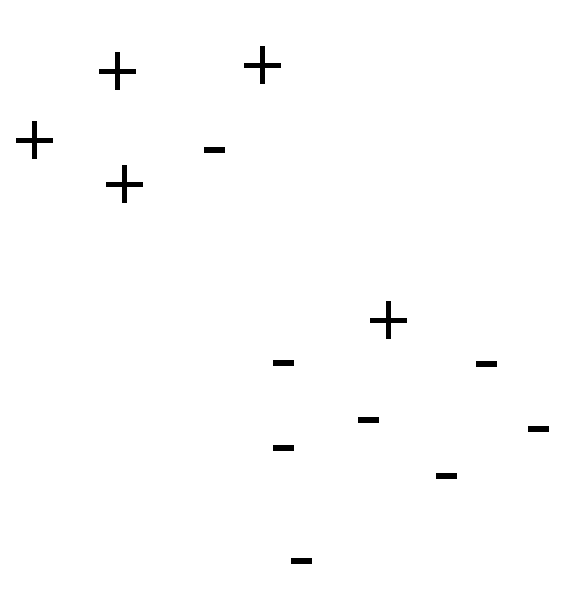
\includegraphics[width=1\textwidth]{lectSVM/nonLinSep.pdf}
\end{column}
\end{columns}

\end{frame}
%***********************************************************
\begin{frame}{``Soft Margin'' Formulation}

\begin{itemize}
\item Go back to the optimization function and add in a ``slack'' variable
\begin{itemize}
\item Choose $w$ to minimize $||w||^2 + c \sum_i \epsilon_i$
\item Subject to $y_i (w \cdot x_i - b) \geq 1 - \epsilon_i$
\item Add a \underline{cost}, $\epsilon$, so the learner doesn't put everything on the wrong side
\item Ideally, $\epsilon$ is 0
\item $c$ is a user supplied variable - it tells the learner how significant a misclassification is
\end{itemize}
\item The ``slack'' needs to appear in both the objective function and in the constraint
\item That's all a soft-margin SVM is!
\vspace{1em}
\item This is a classic approach to handling non-linearly separable data
\end{itemize}
\end{frame}
%***********************************************************
\begin{frame}{How To Solve?}

\begin{itemize}
\item How do we determine $w$ and $b$?
$$w \cdot x - b = 1$$ 
$$w \cdot x - b = -1$$ 
\item Choose $w$ to minimize $||w||^2 + c \sum_i \epsilon_i$
\item Subject to $y_i (w \cdot x_i - b) \geq 1 - \epsilon_i$

\item This is a constrained optimization problem
\end{itemize}
\end{frame}
%***********************************************************
\begin{frame}{Rewrite as an Unconstrained Problem}

\begin{itemize}
\item How do we determine $w$ and $b$?
$$w \cdot x - b = 1$$ 
$$w \cdot x - b = -1$$ 
\item Choose $w$ to minimize $||w||^2 + c \sum_i \epsilon_i$
\item Subject to $y_i (w \cdot x_i - b) \geq 1 - \epsilon_i$

\item Minimize
	$$\frac{\lambda}{2}||w||^2 + \frac{1}{n} \sum_i \max(0, 1 - y_i (w \cdot x_i))$$
	\item where $\lambda = \frac{1}{n \times c}$
	\item $n$ is the number of points
	\item $c$ is the cost from the previous slide
	\item Amenable to gradient descent (one issue: non-smooth max function)
\end{itemize}
\end{frame}
%***********************************************************
\begin{frame}{Non-smooth Max Function}

\begin{columns}
\begin{column}{0.6\textwidth}
\begin{itemize}
\item Can't take the derivative at the max
\item In practice it doesn't matter
\item Ignore those cases
\end{itemize}
\end{column}
\begin{column}{0.4\textwidth}
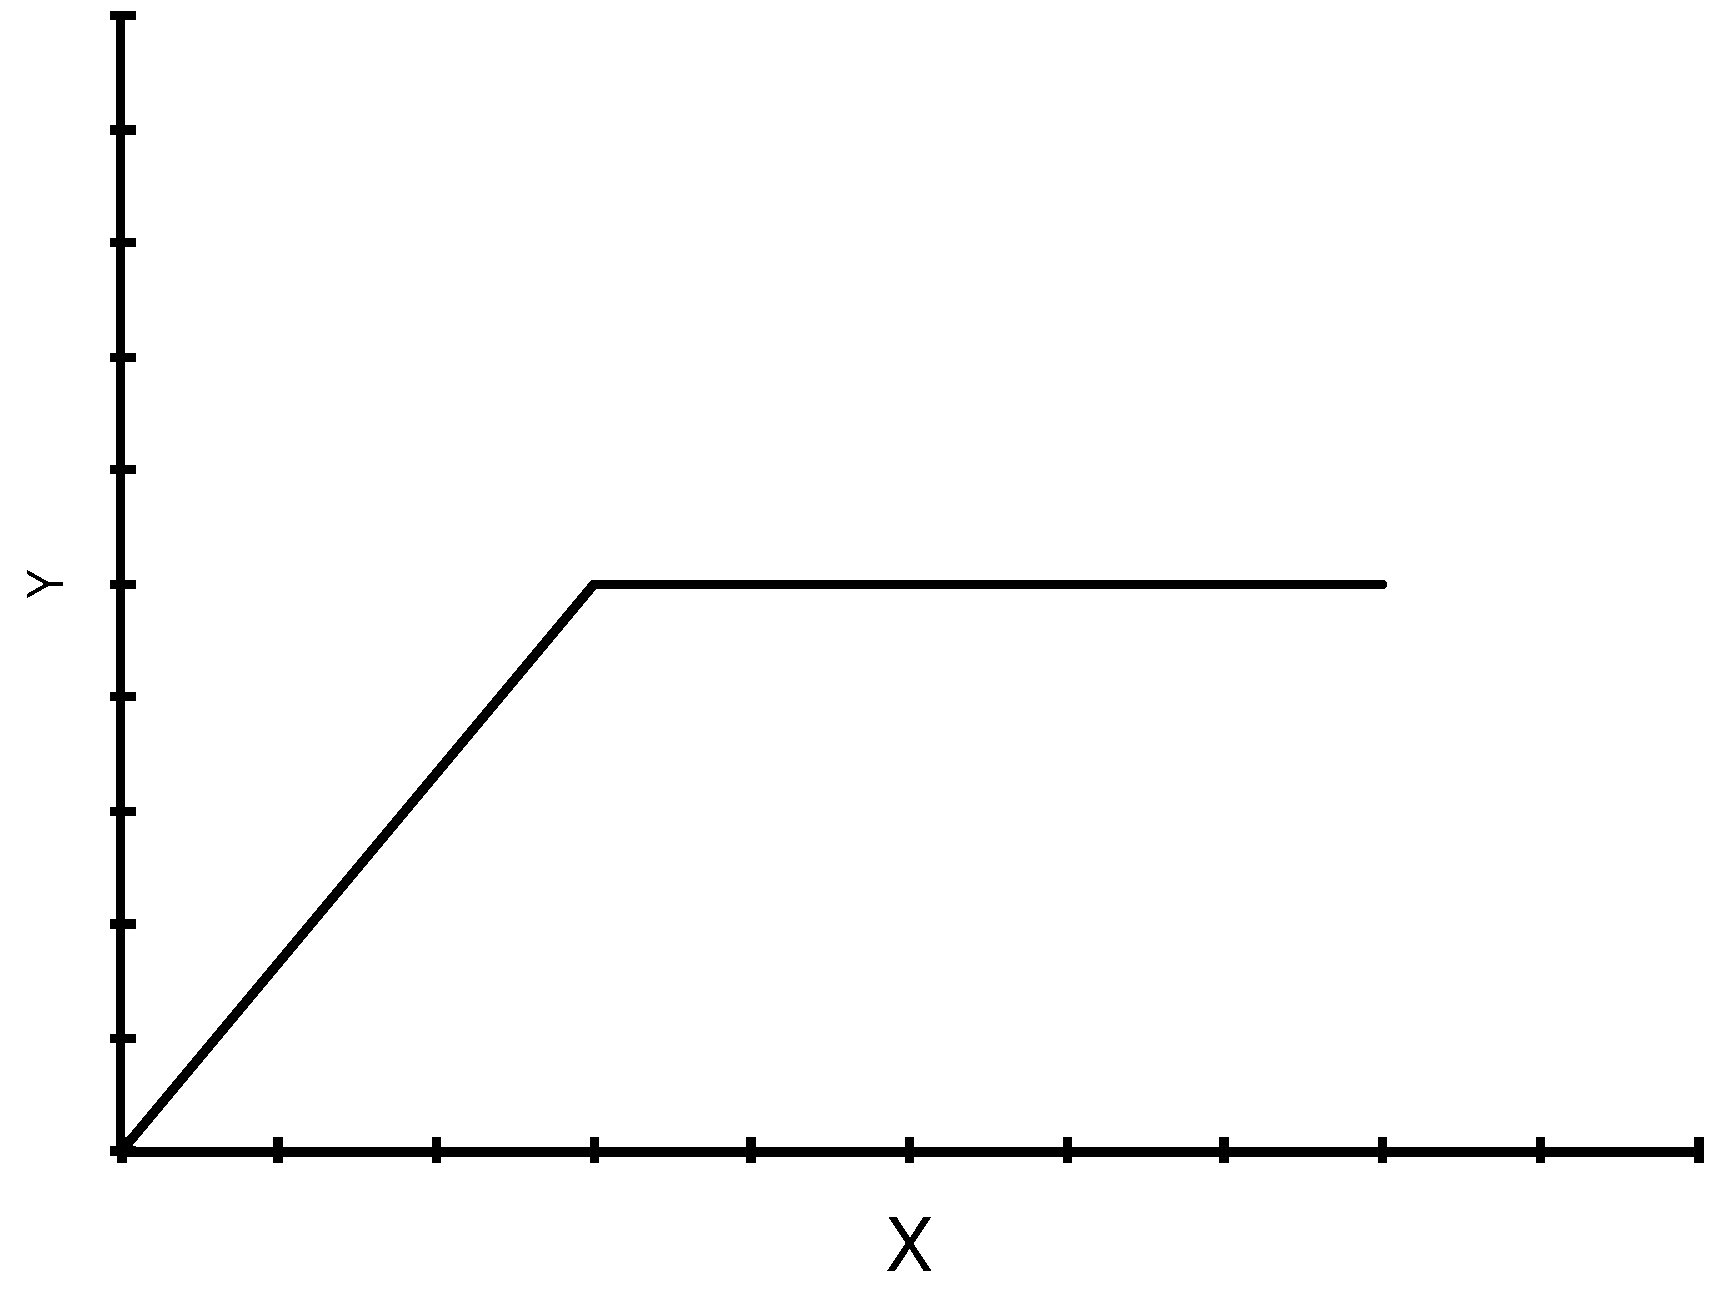
\includegraphics[width=1\textwidth]{lectSVM/maxF}
\end{column}
\end{columns}
\end{frame}
%***********************************************************
\begin{frame}{The Kernel Trick}

\begin{itemize}
\item Motivation:
\begin{itemize}
\item SVMs (and logistic regression) are linear
\item But many classification problems are not...
\item Kernel trick idea: map into higher-D, use linear classifier there
\item Not just for SVMs, but closely linked with them
\end{itemize}
\end{itemize}
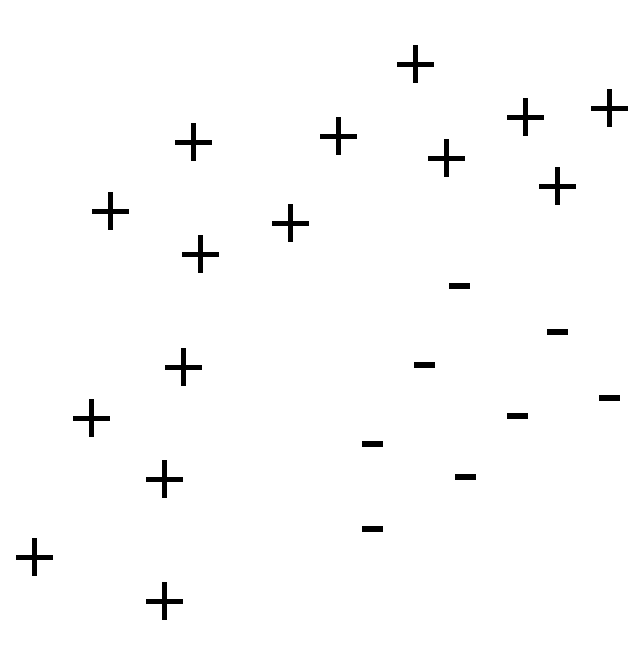
\includegraphics[width=.2\textwidth]{lectSVM/kernel1.pdf} \hspace{2em}
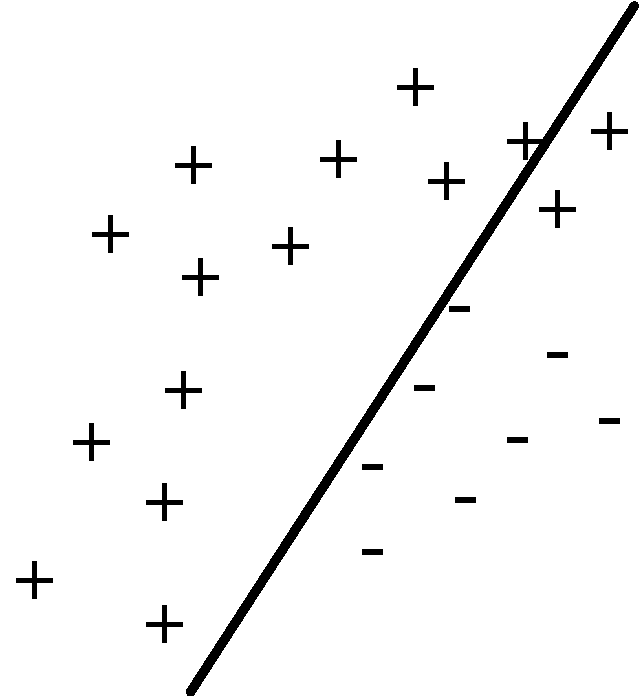
\includegraphics[width=.2\textwidth]{lectSVM/kernel2.pdf}\hspace{2em} % could approximate like this, but that's not what a human would do
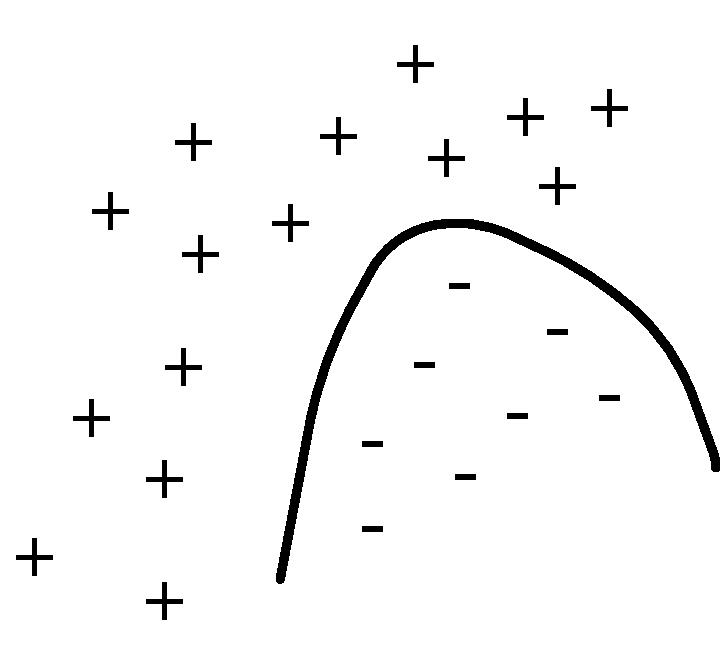
\includegraphics[width=.2\textwidth]{lectSVM/kernel3.pdf} % this is what a human would do


\hspace{4em}Data \hspace{6em}Machine \hspace{6em}Human \\
\end{frame}

%***********************************************************
\begin{frame}{The Kernel Trick}

\begin{itemize}
\item Biggest motivation for SVMs
\item If the number of dimensions $\gg$ number of data points, SVM can build a good classifier
\item Consider the case of periodic data, perhaps a photovoltaic sensor\\
\vspace{1em}
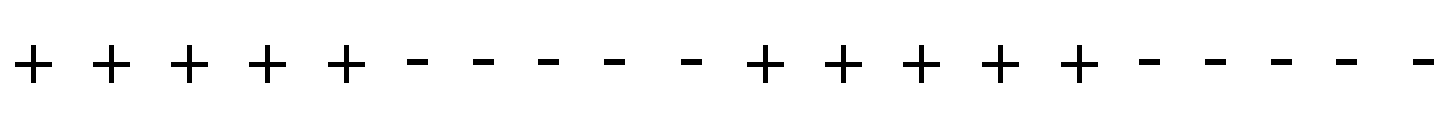
\includegraphics[width=.4\textwidth]{lectSVM/sine1.pdf} \hspace{2em}
\vspace{1em}
\item Clearly, the data are not linearly separable
\item So, map to 2D space by adding a sine value
\item Now, the data are linearly separable

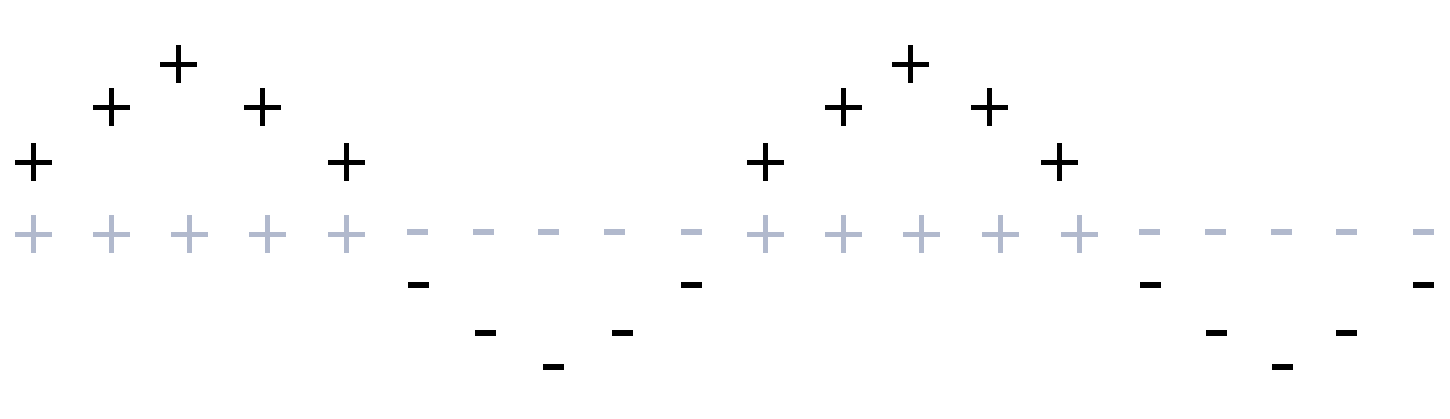
\includegraphics[width=.4\textwidth]{lectSVM/sine2.pdf}\hspace{2em}
\end{itemize}


\end{frame}
%***********************************************************
\begin{frame}{Kernels}

\begin{itemize}
\item Projections that maps the data into a higher dimension space where they are linearly separable
\item This approach can be used with any sort of classifier
\item SVMs are synonymous with kernel methods
\end{itemize}


\end{frame}
%***********************************************************
\begin{frame}{What is a Kernel?}

\begin{itemize}
% this is about mapping point pairs
% think about the mapping to Log space - the important properties are preserved
\item Math tells us:
	\begin{itemize}
	\item ANY mapping from vector pairs to matrix entries...
	\item ...Is equivalent to embedding vectors in SOME high-D space
	\item Where $x'_i \cdot x'_j$ is the matrix entry at $i,j$
	\item As long as we get a  positive semi-definite matrix
	\end{itemize}
\item This mapping is called a ``kernel''
\vspace{1em}
\item Given $n$ points, the pairwise dot products $\rightarrow$ a Positive Semi-definite Matrix
\item Given $n$ points, the pairwise dot products $\leftarrow$ a Positive Semi-definite Matrix \\
in some space
% this can be proven

\end{itemize}
\end{frame}
%***********************************************************
\begin{frame}{The Actual ``Trick''}

\begin{itemize}
\item \textbf{It's possible to learn an SVM without explicitly performing the mapping}
\item Have
	$$\frac{\lambda}{2}||w||^2 + \frac{1}{n} \sum_i \max(0, 1 - y_i (w \cdot x_i))$$
	\item where $\lambda = \frac{1}{n \times c}$
\item To do this, start with the ``dual'' formulation of the problem:
\begin{itemize}
	\item Maximize $$\sum_i \alpha_i \frac{1}{2} \sum_{i,j} \alpha_i \alpha_j (x_i \cdot x_j)$$
	\item Subject to $$0 \leq \alpha_i \leq \frac{1}{\lambda}$$
	\item where $\lambda = \frac{1}{n \times c}$

\end{itemize}
\item We want to choose the $\alpha$s
%\item Key observation: each $x_i$ is \textbf{only} used as input to dot product
%\item So no need to explicitly map to high-D
%	\begin{itemize}
%	\item As long as have the $n$ by $n$ matrix
%	\item Where each entry is pairwise dot product in high-D, we're good!
%	\item We know that the mapping to the high-D space exists % can even be a mapping to an infinite space, where ALL data are linearly separable
%	\end{itemize}
\end{itemize}
\end{frame}
%***********************************************************
\begin{frame}{The Actual ``Trick''}

\begin{itemize}
\item \textbf{Learn an SVM without explicitly performing the mapping}
\begin{itemize}
	\item Maximize $$\sum_i \alpha_i \frac{1}{2} \sum_{i,j} \alpha_i \alpha_j (x_i \cdot x_j)$$
	\item Subject to $$0 \leq \alpha_i \leq \frac{1}{\lambda}$$
	\item where $\lambda = \frac{1}{n \times c}$

\end{itemize}
\item We want to choose the $\alpha$s
\item Key observation: each $x_i$ is \textbf{only} used as input to dot product
\item So no need to explicitly map to high-D
	\begin{itemize}
	\item As long as have the $n$ by $n$ matrix
	\item Where each entry is pairwise dot product in high-D, we're good!
	\item We know that the mapping to the high-D space exists % can even be a mapping to an infinite space, where ALL data are linearly separable
	\end{itemize}
\end{itemize}
\end{frame}
%***********************************************************
\begin{frame}{Standard Kernels}

\begin{itemize}
\item ``Polynomial kernel''
	\begin{itemize}
	\item Replace $(x_i \cdot x_j)$ with $(1 + (x_i \cdot x_j))^d$ for $d > 0$
	\end{itemize}
\item ``Gaussian kernel''
	\begin{itemize}
	\item Replace $(x_i \cdot x_j)$ with $\exp (-|| x_i - x_j ||^2 / (2 \sigma^2))$
	\end{itemize}
\end{itemize}
\end{frame}
%***********************************************************
\begin{frame}{Kernel Trick Plus/Minus}

\begin{itemize}
\item Good: can give better classification accuracy
	\begin{itemize}
	\item Often used in practice for this reason!!
	\end{itemize}
\item Bad: often sensitive to kernel parameter(s) ($\sigma$ in Gaussian kernel, for example)
\item Bad: computationally more complex... 
	\begin{itemize}
	\item Dual formulation not easily amenable to gradient descent
	\item Means kernels useful mostly for smaller problems
	\end{itemize}
\end{itemize}
\end{frame}
%***********************************************************
\begin{frame}{Which Kernel?}

\begin{itemize}
\item Try different ones and compare % "empirically determined"
\end{itemize}
\end{frame}
%***********************************************************
\begin{frame}{Finally: Log Regression,  SVM, or Deep Learning?}

\begin{itemize}
%\item SVM naturally regularizing
\item Have small data, well featurized
	\begin{itemize}
	\item SVM is one of the top options % random forest is right up there
	\item $O(n^2)$ calculations to compute the matrix for the kernel trick
	\item Gets unwieldy after about 50K points
	\end{itemize}
\item Have ``big data'', well featurized
	\begin{itemize}
	\item Regularized Logistic Regression 
	\item Works well
	\item Inexpensive to train
	\end{itemize}
\item Regularized Logistic Regression is comparable to SVM \textbf{without} the kernel trick
\item Have ``big data'' and/or no features
	\begin{itemize}
	\item e.g. text, images
	\item Deep Learning
	\end{itemize}
\end{itemize}
\end{frame}
%***********************************************************
\begin{frame}{Questions?}
\begin{itemize}
	\item What do we know now that we didn't know before?
	\vspace{5em}
	\item How can we use what we learned today?
\end{itemize}
\end{frame}
%***********************************************************
\begin{frame}{Questions?}
\begin{itemize}
	\item What do we know now that we didn't know before?
	\begin{itemize}
		\item SVM is an ML model for classification
		\item It can handle non-linearly separable data
		\item There's a kernel trick that helps us do this
	\end{itemize}
	\item How can we use what we learned today?
	\begin{itemize}
		\item We can use SVM instead of another classification method
	\end{itemize}
\end{itemize}
\end{frame}


\end{document}
